\documentclass[a4paper,12pt,final]{article}
\usepackage[english,french]{babel}
\usepackage[utf8]{inputenc}
\usepackage[T1]{fontenc}
\usepackage[pdftex]{graphicx}
\usepackage[french]{varioref}
\usepackage{times}

\title{English: Explanation of a diagram from the presentation}
\author{ABAK-KALI Nizar\\
   Paris 6 UPMC,\\
   \texttt{nizarabakkali93@gmail.com}}
	
   
\date{\today}
 


\begin{document}
\maketitle
\newpage

\begin{figure}[t]
	  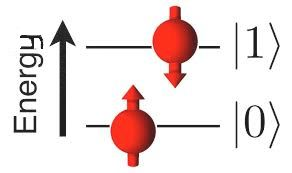
\includegraphics[scale=1.0]{figures/qspin_.png}
	 \caption{A diagram showing two quantic particle and their energetic states}
 
\end{figure}

This diagram was introduced in the second part of the presentation. It was used to explain how quantum bits work. The image show two particules with two arrows pointing in a directions. Furthermore, we can also observe two level ( zero and one ) . \\
the two particules are quantic particules, which means they are very tiny particule that don't follow general physics laws . These particules follow their own rules, the quantic rules. The two arrows correspond to the direction of the magnetic field of the particle that turn . If the arrow is "up" we says that the particle is in the zero state whereas if the arrow is "down" the state is equivalent to one . The state can be set if we control the electrical energy of a particule changing it from up to down at will .



\end{document}
